\documentclass[12pt, a4paper,twoside]{tesi_upf}


\usepackage[latin1]{inputenc}
\usepackage[T1]{fontenc}


%IDIOMES
\usepackage[english,catalan]{babel}
\usepackage[cam,a4,center,frame]{crop}
\usepackage[colorlinks=false]{hyperref}
\usepackage{graphicx}
\usepackage{mathtools}
\usepackage{csquotes}
\usepackage{times}
\pagestyle{plain}
\usepackage[backend=biber,backref,url=false,bibencoding=utf8,sorting=none]{biblatex}
\usepackage{biblatex}
\usepackage{makeidx}
\usepackage{subcaption}
\usepackage{enumitem}
\usepackage{url}
\makeindex


%\bibliographystyle{apalike}
\setlength{\parindent}{1em}
\setlength{\parskip}{1em}



\selectlanguage{catalan}


\addto\captionscatalan
  {\renewcommand{\contentsname}{\Large \sffamily Sumari}}
\addbibresource{../bibliography/bibliography_tesis.bib}
\addbibresource{../bibliography/library.bib}


\title{El titulo de la tesi: In-silico methods to drug discovery}
\subtitle{El subtitulo de la tesi: Cancer}
\author{Autor: Francisco Mart\'inez Jim\'enez}
\thyear{L'any de la tesi: 2016}
\department{Departament: Biomedicine}
\supervisor{Director: Marc A. Marti-Renom}


\begin{document}

\frontmatter


\maketitle

\cleardoublepage




\noindent A mi madre. 

\cleardoublepage





\noindent {\Large \sffamily Agradecimientos} Agraeixo....

\cleardoublepage



\selectlanguage{english}
\section*{\Large \sffamily Abstract}
This is the abstract of the thesis in English.  Please, use less
than 150 words.

\selectlanguage{catalan}
\vspace*{\fill}
\section*{\Large \sffamily  Resum}

Vet aqui el resum de la tesi en catala.  
\vspace*{\fill}

\cleardoublepage


%PREFACI OPCIONAL. SI NO ES VOL, COMENTEU FINS EL FINAL DE PREFACI
{\bf Prefaci}

\cleardoublepage
%FINAL DE PREFACI



\tableofcontents


\listoffigures

\addcontentsline{toc}{chapter}{Index of figures}


\listoftables

\addcontentsline{toc}{chapter}{List of tables}


\mainmatter

\chapter*{Summary}

sencillo

Consta de
\begin{description}
\item[tesi-upf.cls]{\tt book} 
  \begin{enumerate}
  \item Es redissenya la portada  \verb+\maketitle+).

  \item 

  \item Es redefineix {\tt cleardoublepage} para que las paginas en blanco no se numeren
  \end{enumerate}

\item[Preambulel] 
 

\item[paquets] {\tt crop} i {\tt geometry}. 




\item[Taules] Includes \verb+figure+ i un \verb+tabular+ 

\end{description}


\section*{Index}


\begin{enumerate}
\item lo llamas en preambulo  \verb+\usepackage{makeidx} \makeindex+ con esto lo imprimes \verb+\printindex+ con esto lo creas  \verb+makeindex+ 
\end{enumerate}



\chapter{Introduction} \label{introduction} 

\section{Protein are essential molecules}




\par The importance of proteins in biological chemistry is just reflected by their name, derived from the Greek word \textit{proteios}, and that means "of the first rank"\footnote{The term protein was coined by Jons Jacob Berzelius in 1838. It was first used by Gerardus Johannes Mulder, advised by Berzelius, in its publication  \textit{Bulletin des Sciences Physiques et Naturelles en N\'eerlande (1838). pg 104. SUR LA COMPOSITION DE QUELQUES SUBSTANCES ANIMALES}, where he observed that all proteins seemed to have the same empirical formula and came out to the erroneous idea that they might be composed of a single type of very large molecule. Berzelius proposed the name because the material seemed to be the primitive substance of animal nutrition that plants prepare for herbivores.}. Their presence is so essential that they  constitute most of the cell dry mass \cite{kessel2010}. They are not only the cell's building blocks, but also they perform nearly all the cell's functions. Some roles of proteins include serving as structural components of cells and tissues (e.g., \textit{keratin} or \textit{collagen}), transmission of information between cells by hormones such as the \textit{insulin} or the \textit{oxytocin}, facilitating the transport and storage of small molecules (e.g., the transport of oxygen by \textit{hemoglobin}) or providing a defense against foreign invaders (e.g., antibodies). Other proteins such as the \textit{actin} and the \textit{myosin} are responsible of muscle contraction and therefore our movement. However, the most fundamental role of proteins is their ability to act as enzymes, which, catalyzes most of the chemical reactions in biological systems. In summary, proteins are crucial macromolecules present in most of the processes carried out by the cell and, in spite of being extensively studied for many years, they still have many unanswered questions.    
%\par There is experimental evidence of more than 30,000 human protein products derived from over 17,000 human genes \cite{human2014}. That means that each gene expresses on average nearly two different protein \textit{isoforms}.  However, not all the proteome is simultaneously expressed. Estimates say that there are between 8,000 and 9,000 genes expressed in all tissues (i.e. the housekeeping proteome)   

\subsection{Protein structure}

\par A protein is a molecule made from a long chain of amino acids linked thorough a covalent peptide bond. Proteins are therefore also known as \textit{polypeptides}. Attached to this repetitive chain are those portions of the amino acids that are not involved in the covalent bond, the \textbf{side chains}. Side chains confer the different physico-chemical properties of each of the 20 types of amino acids \cite{thecell2008}. The composition of the amino acid sequence determines the function and the structure of a protein. That is because the unique sequence creates a specific pattern of attractive and repulsive forces between amino acids along the polypeptide that leads to a folding process resulting in a specific three-dimensional structure. These forces are usually non-covalent  interactions between the side chains of the amino acids. Non-covalent interactions are weaker than covalent ones, allowing the folded structure to certain degree of  conformation mobility i.e: to be dynamic. This phenomenon is really important to facilitate the interaction with other molecules as we will explore further in \ref{ligand_intect}.  
\par Protein structures are complex conformation of atoms organized in a hierarchical manner \ref{fig:hierarchy_figure}. The first level of this hierarchy, referred to as the \textbf{primary structure}, is the ordered sequence of amino acids of the polypeptide. Certain segments of these chains, tend to form simple shapes such as helices, strands, turns or loops.  These folding patterns are referred to as secondary elements and collectively constitute the \textbf{secondary structure} of the protein. The two most frequent type of secondary elements are the $\alpha$-helixes and the $\beta$-sheets \cite{DSSP}. The overall chain tends to fold further into a three-dimensional  \textbf{tertiary structure}. Contrary to the secondary structure, the tertiary structure folding is driven by interactions from amino acids far apart in the primary sequence. The tertiary structure, is generally the most stable form of the protein, that is, the one that minimizes its free energy \cite{Dill1990}. Furthermore, the tertiary structure is also the biologically active form of the protein, and its unfolding usually leads towards partial o total inactivation of the protein. Finally, some proteins are composed by multiple folded chains. In such cases, each folded subunit folds independently and then joins the others forming a biologically active complex. This type of organization is considered as the \textbf{quaternary structure}.
\begin{figure}[h]

  \centering
  	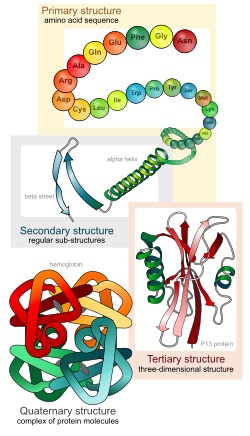
\includegraphics[scale=0.75]{../figures/protein_structure_levels_en.png} % Figure was taking from...

	\caption{Hierarchical distribution of layers in protein structure}
	\label{fig:hierarchy_figure}
\end{figure}
\par This traditional paradigm of protein structure has been challenged by some exceptions of proteins that lacks of a fixed or ordered three-dimensional structure. The intrinsically disordered proteins (IDPs) cover a wide spectrum of states from fully unstructured to partially structured including conformations such as \textit{random coils} or \textit{molten globules}. Moreover, some  factors may lead to the permanent loss of structure of a protein, and when that occurs, they endanger the entire organism. How problematic protein misfolding can be for the organism is illustrated by examples such as cystic fibrosis, Alzheimer's, Parkinson's and Huntington's diseases.
\par Figure \ref{fig:strucrure_sequence_figure} from the seminal paper \cite{StructureSequence} shows the correlation degree to which protein structures changed as a function of sequence divergence. This work helped to set up the fundaments of what is considered a central paradigm in protein evolution: protein structure is more conserved than sequence. However, not all the regions in a protein structure are equally conserved. It's been shown that functionally important amino acids, responsible of the interaction with other molecules, are more conserved than the rest of the protein structure \cite{conservPPI}. Additionally, the structural core is more conserved than the surface \cite{Raj2007}. The high conservation of the core enables the protein to maintain the global shape, while the surface is free to change (i.e.to mutate) some functional features \cite{Todd2001}.   These evolutionary mechanism are in accordance with the central \textit{sequence $\rightarrow$ structure $\rightarrow$ function} paradigm that prevails in the protein evolution field. 

\begin{figure}[h]

  \centering
  	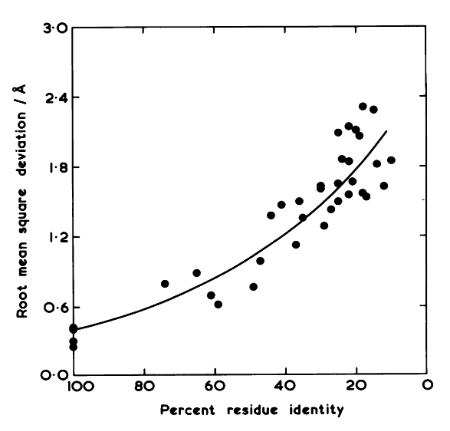
\includegraphics[scale=0.5]{../figures/structure_vs_sequence.png} % Figure was taking from...

	\caption{The original plot of the relation of residue identity and the r.m.s. deviation of the backbone atoms of the common cores of 32 pairs of homologous proteins. Figure extracted from \cite{StructureSequence}}
	\label{fig:strucrure_sequence_figure}
\end{figure}
 
\subsubsection{Protein Structure Determination}

\par Since in 1960, the Brithis biochemist John Kendrew determined the myoblobin structure \cite{KENDREW1960}, more than 37,000 different protein structures have been deposited in the Protein Data Bank (PDB) \cite{Berman2000}. The PDB is a repository created in the 1970s with the aim of storing all the 3D protein structures and unifying their format. Figure \ref{fig:structures_pdb} shows the variation of the number of deposited structures over the time. The number of PDB structures has significantly been increased over the last years thanks to initiatives such as the Protein Structure Initiative (PSI) \cite{Norvell2007} or the structural genomics \cite{GIleadi2007}. The later, was born with the aim of determining the structure of all human proteins. However, soon after, they realized that the goal was unrealistic. Fortunately, the number of folds which represent the complete \textit{fold space} observed in nature is much smaller that the number of proteins. Therefore, the current goal is to determine the structure of a representative set of proteins, that is, at least one protein per fold class. Once It is known the structure of one representative protein, and thanks to the \textit{homology modeling} methods, It is usually feasible inferring the structure of other proteins belonging to the same fold class as  we will explore further in the next section \ref{structure_predicion}.
\par Several methods are currently used to experimentally determine the 3D structure of a protein. More than 99$\%$ of structures deposited in the PDB have been determine by the three main methods:  X-ray crystallography, nuclear magnetic resonance  spectroscopy (NMR) and electron microscopy (EM) (Figure \ref{fig:smethods_pie}). These methods provide experimental data that helps the scientist to elucidate the final structure of the protein. However, in most cases, the experimental data is not sufficient by itself to build an atomic model from scratch. Additional knowledge about the molecular structure most be added. For example, the preferred geometry of atoms in a standard protein, the patterns of repulsion and attraction of amino acids, etc. All this information allows the building of the final model that is consistent with both the experimental data and the prior knowledge of the 3D geometry of the molecules. We next briefly explain the three aforementioned methods:

\begin{enumerate}[label=(\alph*)]
\item \textbf{X-ray crystallography}. Currently, it is the most widely used method in protein structure determination. Almost 90$\%$ of the structures deposited in PDB come from X-ray crystallization (Figure \ref{fig:smethods_pie}). In this method, X-rays fired at a crystal of the molecule are diffracted by the electron clouds of the atoms in the crystal, forming an unique pattern that is printed as a picture of the atomic density map. Subsequently, the diffraction pattern is combined with other physio-chemical knowledge of the protein, such as composition or atomic geometrical restrictions, in order to build the final 3D model \cite{Smyth2000}. 
\par Before the X-ray exposition, it is then necessary a prior step of crystallization of the molecule.  Unfortunately, the crystallization step introduces itself a great number of limitations.  The flexibility of proteins is one of the these limitations. The flexible nature of proteins makes really difficult the creation of an accurate and homogeneous alignment of multiple molecules used to create the crystal. Another important limitation is the different conditions required for crystallizing each different molecule. These limitation are especially noteworthy in membrane proteins. Despite of nearly 30$\%$ of eukaryotic proteins are membrane proteins, only 604 unique membrane protein structures have been solved to date (data extracted from \url{http://blanco.biomol.uci.edu/mpstruc/}; date 21-03-2016). As a consequence, alternative innovative developments are needed to overcome the numerous obstacles associated with X-ray structure determination of membrane proteins \cite{Bill2011}. 
\par The accuracy of the final atomic structure relies on the quality of the generated crystals. Two important measures of the accuracy of a crystallographic structure are its atomic \textit{resolution}, which refers to the smallest separation between crystal lattice planes that is resolved in the diffraction pattern \cite{Yaffe2005}, and the \textit{R-factor}, which measures how well the refined structure predicts the observed data \cite{Morris1992}. 

\item \textbf{NMR spectroscopy}. The NMR spectroscopy technique has been used for years to determine the structure of proteins. Currently, almost 10$\%$ of the structures deposited in PDB have been determined by this method (Figure \ref{fig:smethods_pie}). In NMR spectroscopy, the protein is purified, placed in a strong magnetic field, and eventually probed with radio waves. The observed set of atomic resonances is then analyzed to retrieve a list of atomic nuclei that are close in the space. Similarly to X-ray crystallography, this set of restrains is subsequently used to build the structural model of the protein that contains the 3D conformation of each atom in the space \cite{Wider2000}.   
\par NMR spectroscopy has a major advantage over X-ray crystallography: it provides information on proteins in solution. Therefore, this method is the main method for studying the atomic structure of highly flexible proteins. A standard NMR structure includes an ensemble of protein structures, all of them being consistent with the experimentally observed set of restraints. The ensemble of structures are very similar in those regions with strong restrains, less constrained regions of the proteins, on the other hand, show less agreement in the generated models. These lack of restriction areas are presumably the flexible regions of the protein since they do not provide a strong signal in the experiment.   
\par A big limitation in comparison with X-ray crystallography is its applicability: this technique is usually limited to proteins smaller than 35 kDa. Moreover, NMR can only be applied to soluble proteins that do not aggregate and are stable during the NMR experiment \cite{Wider2000, Gadian1993}. NMR is also inherently insensitive and milligram amount of proteins are required \cite{Gadian1993}. All these limitations have hampered the broader use of this technique narrowing down the cases where this method is fruitful.

\item \textbf{Electron microscopy} methods. EM methods are emerging as a very versatile tool for determining the structure of large macromolecular complexes. To date, less than 1$\%$ of proteins in PDB have been determined by EM methods (Figure \ref{fig:smethods_pie}). However, in recent years there has been dramatic increase in the number of complexes determined by EM technologies. The \textit{revolution} in the structural biology field is perfectly manifested by the cryo-electron microscopy (cryoEM) method: in 2015 alone, cryoEM was used to map the structures of more than 100 different molecules \cite{CryoEM}. In cryoEM a beam of electrons is fired at a frozen protein solution. The
emerging scattered electrons pass through a lens to create a magnified image on the detector, and the structure can then be deduced afterwards. 
\par The utility of cryoEM and others EM tools lies on the fact that it allows the observation of molecules that have not been fixed in any way, showing them in their native environment. This is the opposite of the crystallization step in X-ray crystallography, which many times hampers the success of the whole procedure. CryoEM have been traditionally used in large molecules such as ribosomes\cite{Khatter2015} or the V-ATPase\cite{Zhao2015}, but they have also shown their potential in small membrane proteins\cite{Liao2013} and medically important proteins\cite{Bai2015}. 
\par However, there are still a room for further improvement in EM technologies. Despite of recent advances in the resolution, most of the cryoEM structures have lower resolution than the X-ray ones. Furthermore, there are numerous technical unsolved problems that need to be addressed to make easier its standardization and systematical application. Finally, the high prize of cryoEM experiments are many times  slowing Its spread and therefore, there is a need to reduce cost in order to make it globally accessible. %Mirar identacion
\end{enumerate}
 

\begin{figure}[!tbp]
  
  \centering
    \begin{subfigure}[b]{0.75\textwidth}
	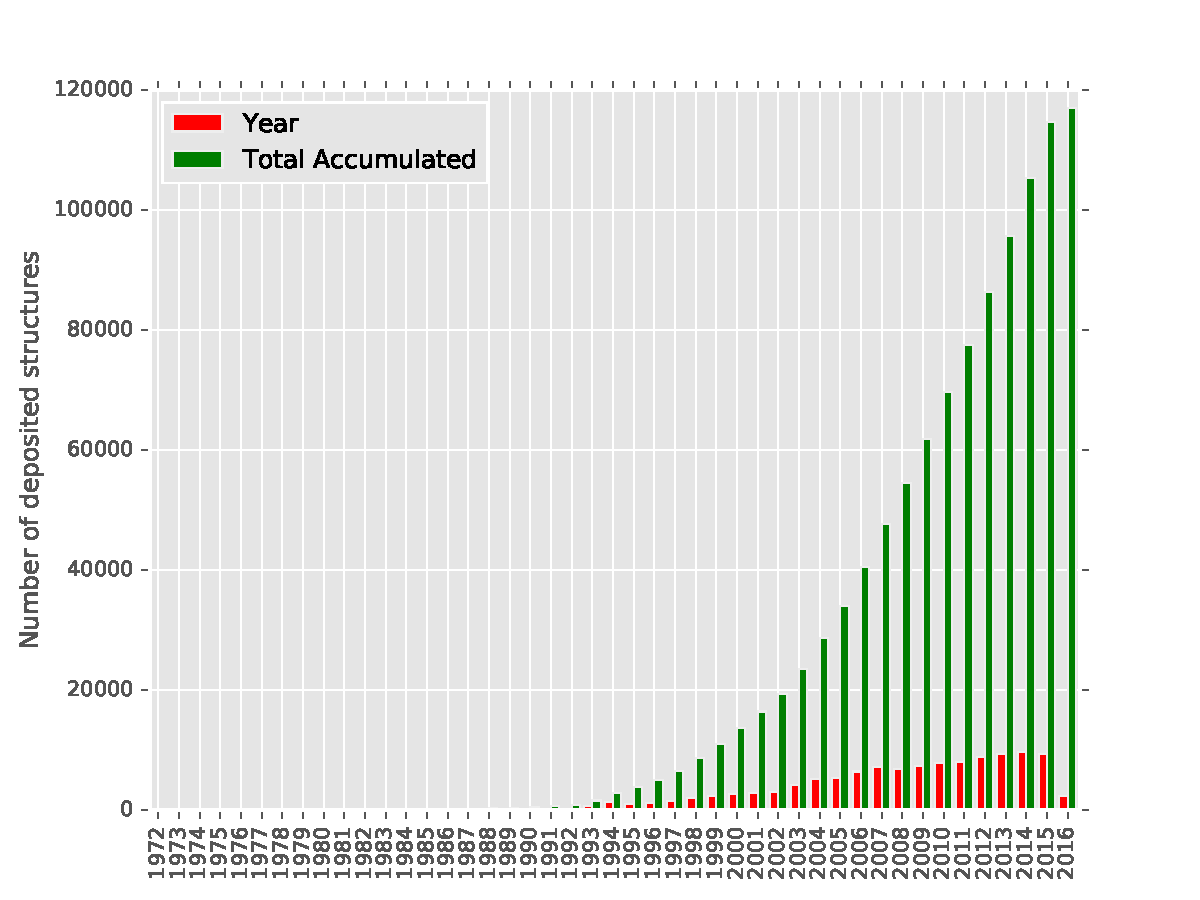
\includegraphics[width=1\linewidth]{../figures/pdbs_per_year.pdf}
	\caption{}
	\label{fig:structures_pdb}
	\end{subfigure}
	\begin{subfigure}[b]{0.55\textwidth}
	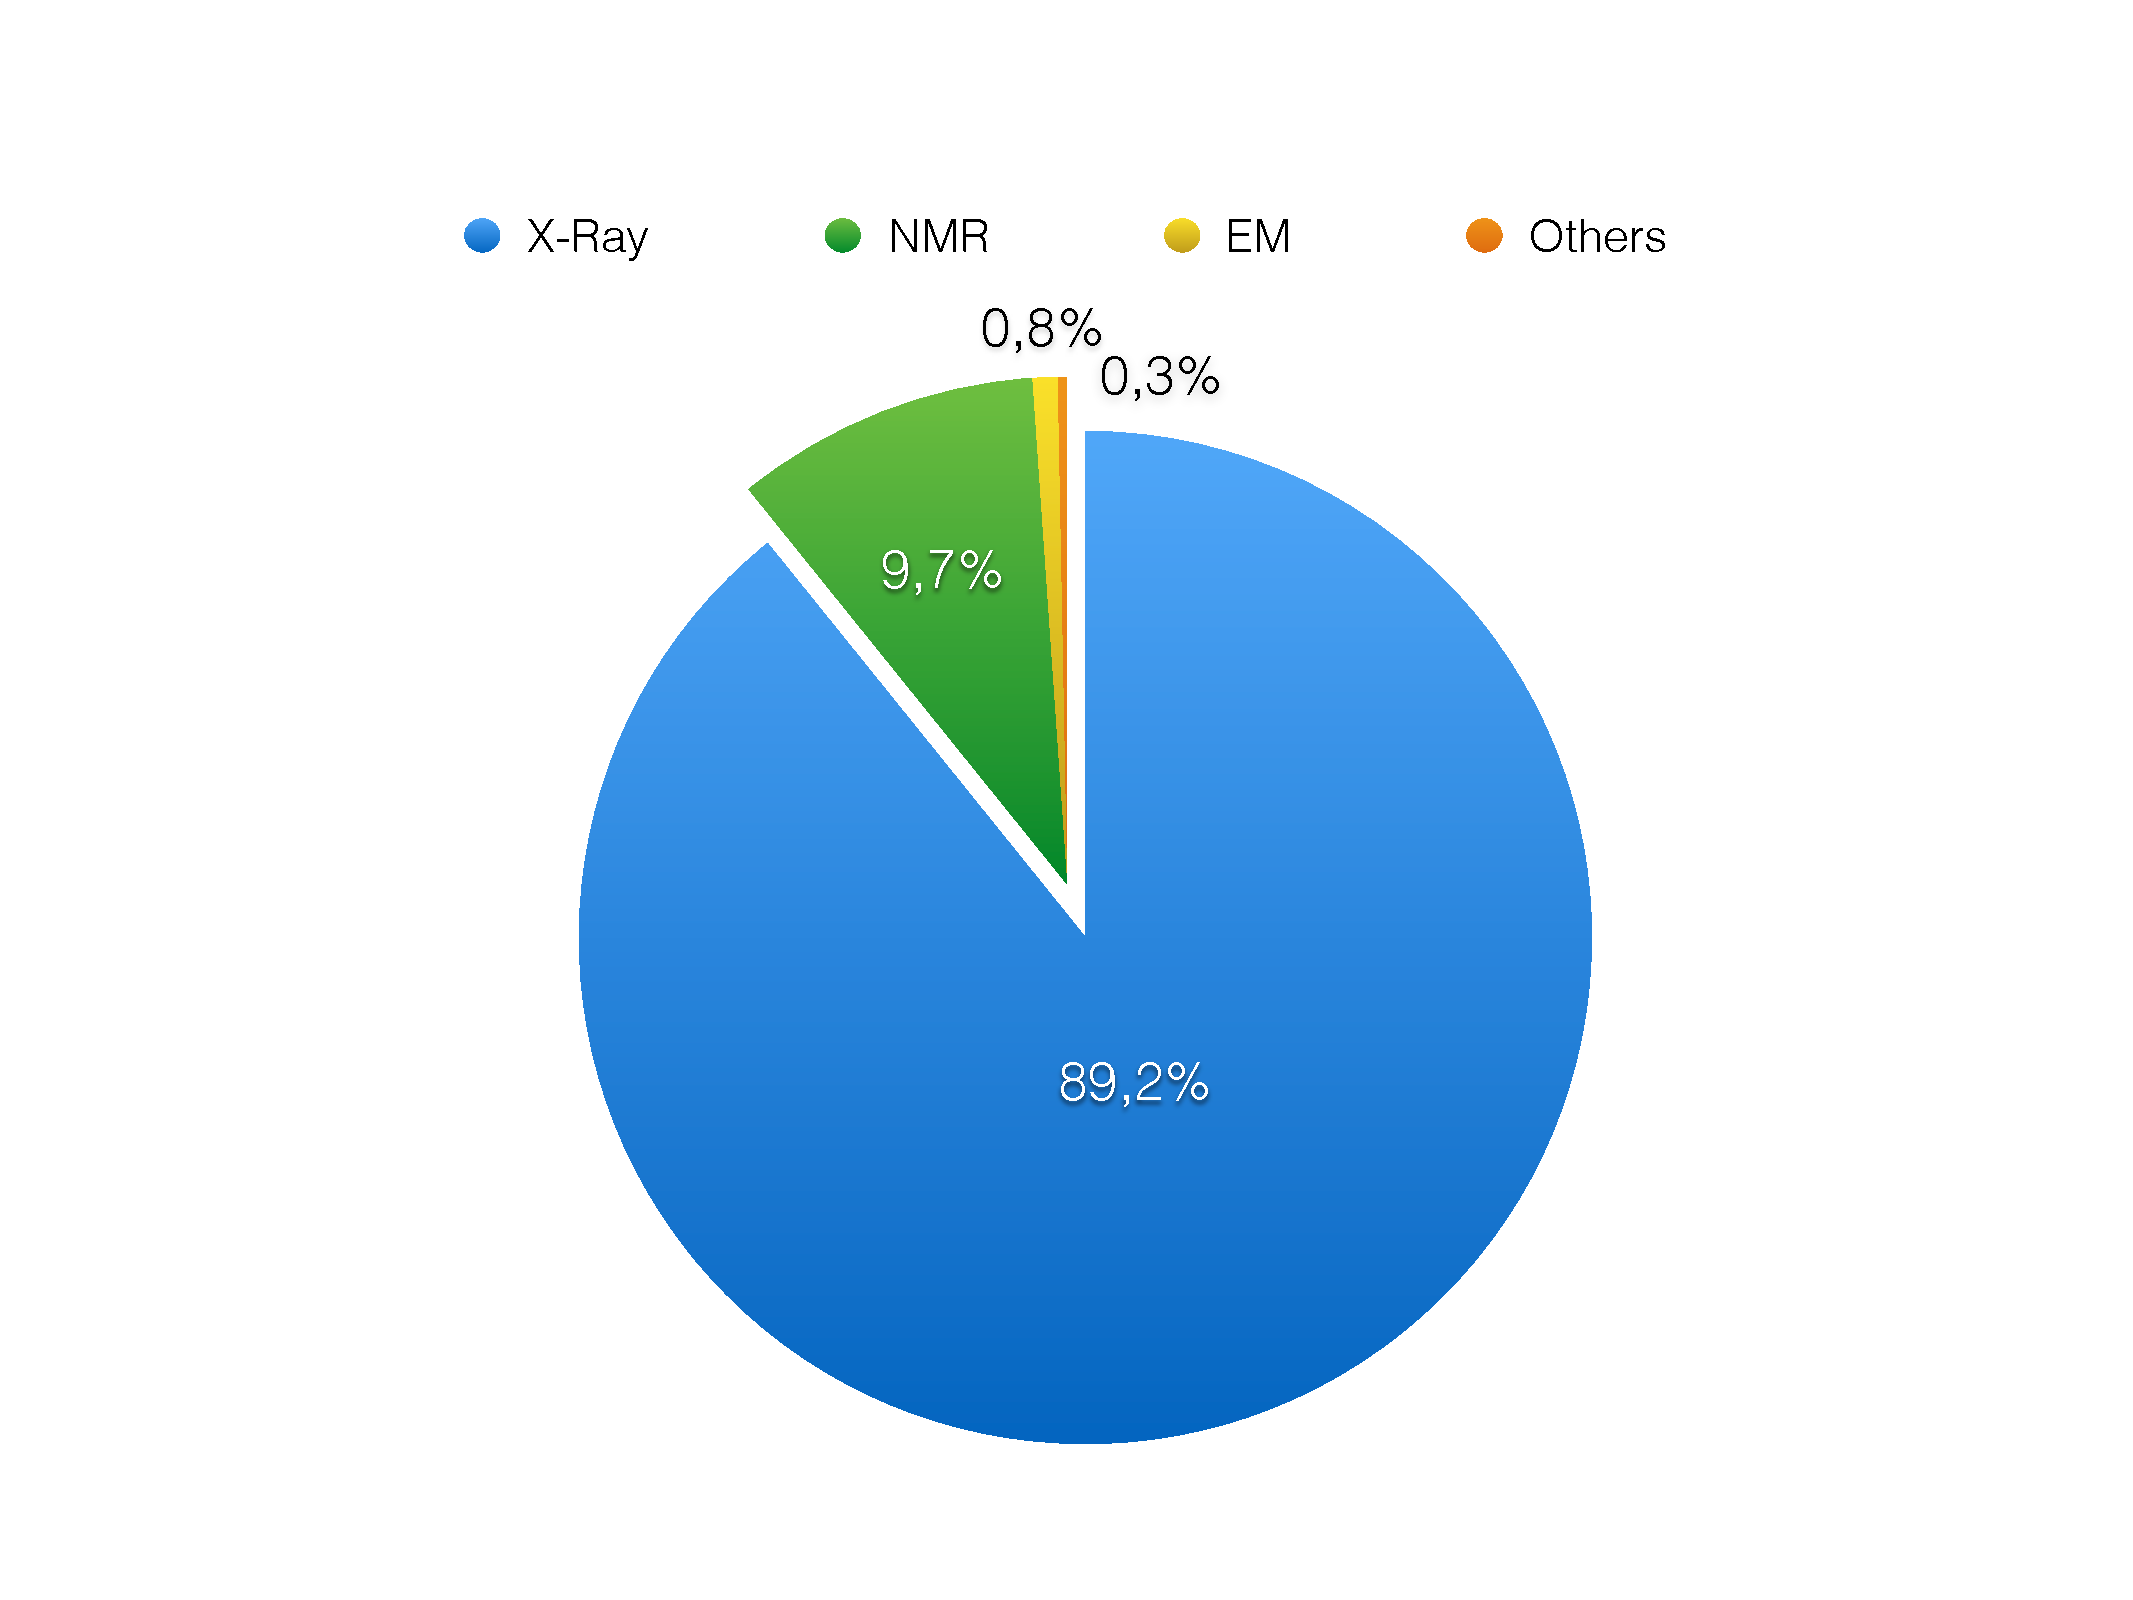
\includegraphics[width=1\linewidth]{../figures/pie_smethods.pdf}
	\caption{}
	\label{fig:smethods_pie}
	\end{subfigure}
   \caption{a) Growth of released structures per year. Data extracted from PDB. b) Pie chart with the percetange of structures determined by the different methods. Data extracted from PDB.}
   
	
	
\end{figure}


\pagebreak

\subsubsection{Protein Structure Prediction} \label{structure_predicion}


\par Despite of the advances in methods for protein structure determination, most of the known proteins lack of structure in the PDB. There are 550,740 annotated and curated protein sequences in UniProtKB (\url{http://www.uniprot.org}, April 2016).  However, only 4$\%$ of them (23,195 different protein sequences) have a link to a PDB structure. Therefore, there is a gap between the number of known protein sequences and the number of determined structures: the \textit{sequence-structure gap}. 
Computational methods for structure determination are helping to bridge this gap. The prediction of the 3D structure of a protein from its amino acid sequence has always been one of the most desirable goals in computational biology. It would save a lot of resources, and it would set a milestone in the structural biology field. Unfortunately, we are still far from being able to predict the structure of any protein from its primary protein sequence. Broadly, for different approaches are commonly used. The first, and most extensively used, is the \textit{homology} or \textit{comparative} modeling, that uses similar experimentally determined structures to model the structure of the protein of interest \ref{Homology_modeling}. Second, \textit{fold recognition} and \textit{threading} methods are used to model protein structures with low similarity to known protein structures \cite{Jones1992, Bowie1991}. Third, \textit{de novo} or \textit{ab initio} methods make their predictions by combining the principles of physics that rule protein folding, with information derived from known structures but without relying in any type of similarity or evolutionary relationship to known folds \cite{Lee2009}. Finally, the \textit{integrative} or \textit{hybrid} methods combines different computational and/or experimental sources to perform the structure prediction \cite{Russel2012}.   
 
\subsubsection{Homology modeling} \label{Homology_modeling}


\par This type of protein structure prediction methods exploits the evolutionary relationship between the \textit{target} protein (i.e. protein being modeled) and the \textit{templates} with known experimental structure. They are based on the biological premise that evolutionary related sequences tend to have similar 3D structures. The usual workflow of homology modeling consist on several consecutive steps: 
\begin{enumerate}
\item \textbf{Identification of suitable template structures related to the target protein}. This step consist on a search for similar sequences with known 3D structure. This task is easy when a close homologue of the target protein has been solved. Initiatives such as PSI\cite{Norvell2007} are helping in this issue in order to increase the number of modellable proteins. However, there are still many proteins with lack of homologous proteins in PDB. In these cases, alternative methods such as \texit{ab initio} should be used.  

\item \textbf{Alignment between the target and the template(s) sequence(s)}. The sequence identity of the target-template alignment is the most frequently used measure for similarity. Consequently, the sequence identity is also a good predictor of the final 3D model quality. The overall accuracy of models calculated form aligments with sequence identity higher than 40$\%$ is usually good (i.e. RMSD\footnote{Root Mean Square Deviation is the measure of the average distance between the atoms of two superimposed proteins. Equation $RMSD=\sqrt[]{\frac{1}{N} \sum\limits_{i=1}^N \delta_i^2}$ where $\delta_i$ is the distance between the $N_i$ pair of equivalent atoms (usually the C$\alpha$).}  lower than 2.0\AA). In the 30$\%$-40$\%$ identity range, errors can be more severe and are often locate in loops and highly flexible regions. Below the 30$\%$ of sequence similarity, often referred to as \textit{twilight region}, serious errors occurs including the basic fold being mis-predicted \cite{Baker2001, twilight1996}.
Figure \ref{fig:homology_modeling} shows an empirical threshold for  homology modeling extracted from \cite{Sander1991}. The region below the curve covers those cases where the alignment does not carry enough information to model the 3D structure, while area above the threshold curve, include those cases where homology modeling is appropriate.  
\item \textbf{Modeling of the structurally conserved regions and prediction of the structurally variable regions.}. There are different algorithms to assign the spatial coordinates of the target protein using the template(s)-target alignment information. Highly conserved regions are generally well modeled, while those regions with insertions or gaps are more prone to include errors and sub-optimal atomic orientations. 

\item \textbf{Refinement of the initial model.} In this step the model is refined to idealize bond geometry and to remove errors that may have been introduced in the modeling step. The refinement process pursues the free energy minimization of the generated 3D protein model. Many different algorithms have been applied to perform the minimization step: molecular mechanics force fields \cite{PRO1410}, molecular dynamics \cite{Fiser2000}, Monte Carlo \cite{Kidera1995} and Genetic Algorithms\cite{McGarrah1993}.
 
\item \textbf{Evaluation of the model(s).} Model evaluation seeks for the identification of the different errors that might have occurred during the modeling process. Numerous methods have been developed to assess the quality of a 3D model. In fact, 3D model assessment has a very such productive field for many years that it was included in the seventh edition of the CASP experiment \cite{PROT21669}. The general question of how accurate is a model can be reformulated by several more specialized questions: 
\begin{enumerate}

\end{enumerate}[label=\roman*]
\item Is the selected fold correct? The fold assessment consist of deciding whether a given protein model has the right fold. Residue-based combined accessible surface and distance-dependent scoring function have shown the best performance in this task \cite{Melo2002}. 
\item How do we select the best model among the set of decoys or alternative solutions? Several models can be generated by making changes in the template-target alignment, by selecting different template(s) structure(s) or by using different seeds in the refinement non-deterministic algorithms. Atom-based distance-depend scoring functions have proved to be useful for this particular task in some cases\cite{Samudrala1998}. However, there is not a gold standard for ranking the generated 3D models. Thus, the model selection eventually relies on the expertise of the person running the modeling. 
\item Which is the overall accuracy of the model? This question can be addressed by defining a score that correlates with the RMSD after superimposing a model and its native structure. AKI
\item Which is the accuracy of the model in particular regions of the model?
\end{enumerate}

\par limitations 

\footnote{For a comprehensive review of homology modeling methods, limitations and applications please consider \cite{Marti-Renom2000, Malmstrom2010} 
\end{enumerate}
\begin{figure}[h]

  \centering
  	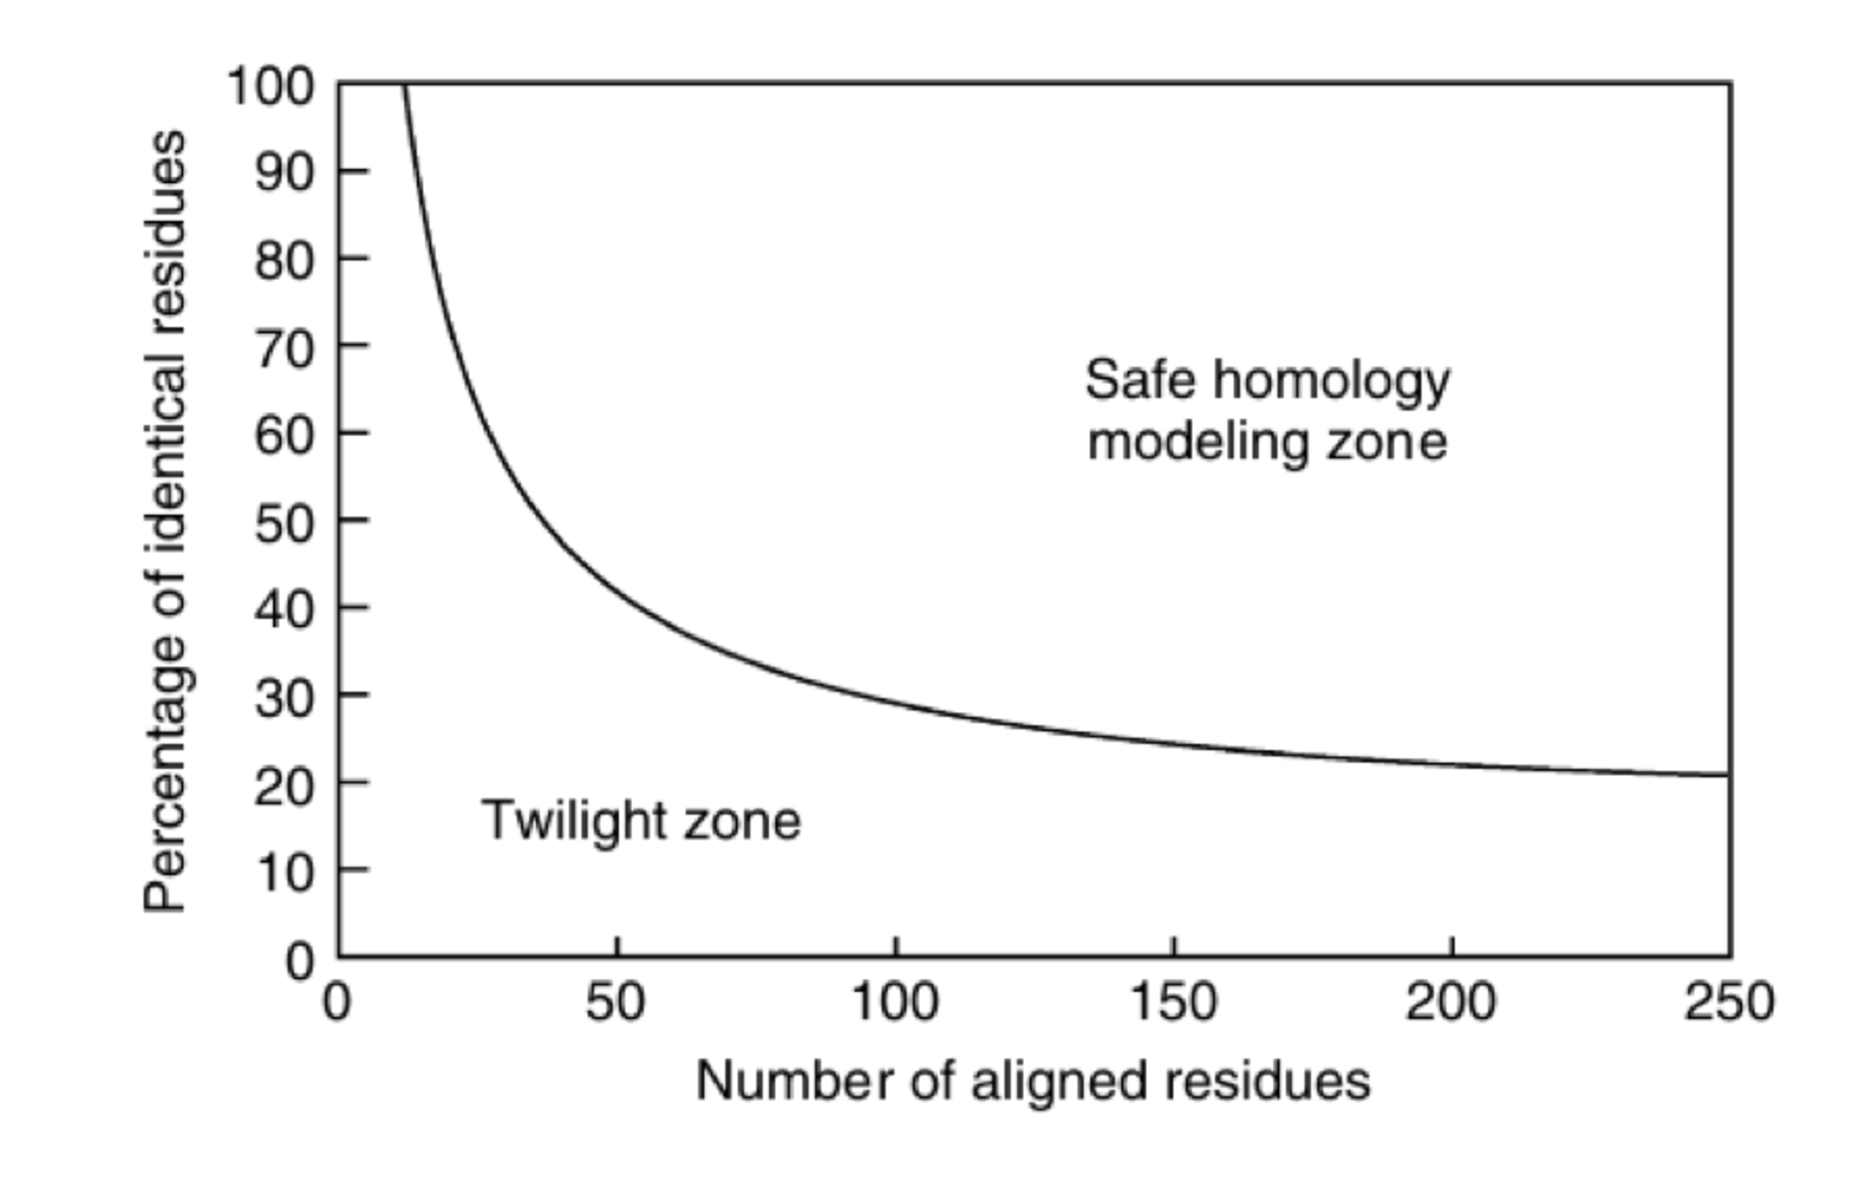
\includegraphics[scale=0.5]{../figures/homology_plot.pdf} % Figure was taking from...

	\caption{Homology threshold curve as a function of alignment length. Data extracted from \cite{Sander1991}}
	\label{fig:homology_modeling}
\end{figure}
Limitations
Examples Modeller 
[Citar libro]

\subsection{Protein function}

\par The major question in the protein biology field has been to understand the protein sequence, structure, function relationship. It is known that structure of a protein determines its biological function. However, different \textit{regions} of the structure can perform semi-indepent functions from each other. These regions are referred to as \textbf{protein domains}. A domain is substructure produced by any part of polypedtide chain that can fold independently into a compact and stable structure \cite{Richardson1981, That1991, DomainDef}. Domains on average contain 80-250 residues \cite{Islam1995}. Estimates of the number of domains per protein say that nire than 70\% of procaryotik proteins and 80\% of eukaryotic proteins include more than one domain \cite{Han2007, Chothia2003}. Among this multi-domain proteins, 95\% of them contains only two to five protein domains \cite{Han2007}.  Domains are not only the basic functional units of proteins, but also the evolutionary units of protein evolution. As proteins have evolved, domains have been modified and combined to build new proteins \cite{Vogel2004, Apic2001}. 
Such is the importance  of domains in protein evolution, that they have been included in current protein classification methods as one of the major classification parameters. Some of these domain classification methods such as SCOP \cite{Murzin1995} or CATH \cite{Orengo1997} are purely based on the structure, while others such as Pfam \cite{Bateman2002} or INTERPRO \cite{Hunter2009} include information about the function in their classification. 
\par Domains, and consequently proteins, perform its biological activity by interacting with other molecules. Proteins can interact with other proteins, constructing a protein-protein complex, with ions or with small-molecules. The substance that is bound to the \textit{target} protein is called the \textbf{ligand}, while the region of the protein where the ligand is binding is called ligand's \textit{binding site}\footnote{For simplicity, in this manuscript, unless otherwise indicated, the term ligand will only refer to small molecules ligands, while proteins ligands will be explicit named as protein-protein interactions}. 



\subsection{Protein-Ligand Interactions} \label{ligand_intect}


\par The roles played by the ligands are diverse. Table X shows an example of the different functions that a small-molecule ligands can perform in a protein. 
Binding constants, allosteric and binding-site, induced fit model. Expandir. Imporatante. 

 




\subsection{Protein-ligand prediction}


\section{Drug discovery}



\begin{table}[h]
  \centering
  \begin{tabular}{|l|l|}
   \hline
    0 & 0 \\ \hline
    0 & 0 \\ \hline    
  \end{tabular}
  \caption{Prova de taula}

\end{table}

\subsection{subsection}
Subsection

\section{Drug discovery}
Second
\subsection{In-silico methods in drug-discovery}
Subsection
\section{Mycobacterium tuberculosis}
\subsection{Tuberculosis treatments and PPcs}
\section{Drug resistance in cancer}
\subsection{Cancer Treatment and drugs}





\chapter{Objectives}
\chapter{nAnnolyze}
\chapter{Predicting targets in MTB}
\chapter{Drug resistance in cancer}



\begin{figure}[b]
  \centering
  
\includegraphics[scale=0.5]{../figures/logo_upf.png}
    \caption{Example}
    \label{fig:logo}
\end{figure}





%\bibliography{/Users/fran/Documents/Work/tesis/bibliography/bibliography_tesis}



\backmatter
\printindex

\printbibliography






\end{document}
